\documentclass{beamer}

\usepackage{graphicx}
\usepackage{listings}
\usepackage{xcolor}
\usepackage{amsmath}
\usepackage{enumitem}
\usepackage{semantic}

\setlist[description]{leftmargin=0in,labelindent=-5pt}

%\lstset{basicstyle={\footnotesize\ttfamily},columns=fullflexible, language=Java} 
\lstset{
         %language=Java,
         basicstyle=\tiny\ttfamily, % Standardschrift
         %numbers=left,               % Ort der Zeilennummern
         numberstyle=\tiny,          % Stil der Zeilennummern
         %stepnumber=2,               % Abstand zwischen den Zeilennummern
         numbersep=5pt,              % Abstand der Nummern zum Text
         tabsize=1,                  % Groesse von Tabs
         extendedchars=true,         %
         breaklines=true,            % Zeilen werden Umgebrochen
         keywordstyle=\bf, %\underline,
         morekeywords={find,in,new,then,let,for,probably,act,self,now,export,else,if,then},
         numbers=left,
         escapeinside={(*}{*)},
         %moredelim=[is][\color{blue}\underbar]{@}{@},
         %moredelim=[is][\bf\underbar]{^}{^},
         literate={Lambda}{$\Lambda$}{1}{rho}{$\rho$}{1}{dots}{$\ldots$}{1}{forall}{$\forall$}{1},
         %deletekeywords={new},
         showspaces=false,           % Leerzeichen anzeigen ?
         keepspaces=true,
         showtabs=false,             % Tabs anzeigen ? 
         showstringspaces=false      % Leerzeichen in Strings anzeigen ?        
 }
 
 \def\code#1{{\normalfont\lstinline[basicstyle=\small\ttfamily]{#1}}}
 \def\new{{\normalfont\lstinline[basicstyle=\small\ttfamily,deletekeywords={new}]{new}} }\definecolor{ao(english)}{rgb}{0.0, 0.5, 0.0}
 \definecolor{britishracinggreen}{rgb}{0.0, 0.26, 0.15}

% \usepackage{beamerthemesplit} // Activate for custom appearance

\title{ESL: Simple Examples}
\author{Tony Clark}
\date{\today}

\begin{document}

\frame{\titlepage}

\frame
{
  \frametitle{Simple Goals}
  \centering
  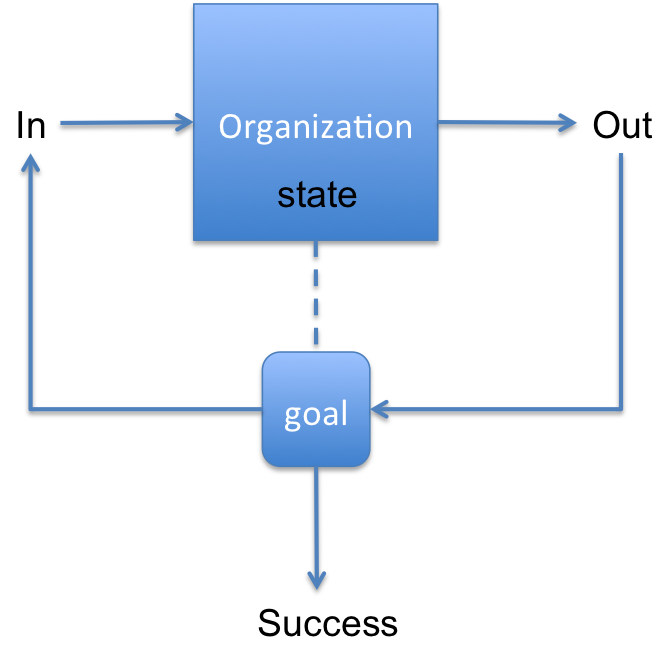
\includegraphics[scale=0.7]{goals}  
}

\begin{frame}[fragile]
  \frametitle{ESL Implementation}
\begin{lstlisting}
export main;                                   // all ESL programs export main.
act main {                                     // main is a behaviour.
  act organization(goal) {                     // the simulated organization.
    state = 0                                  // init state.
    In -> {                                    // simple input event.
      probably(50) state := state + 1 else {}; // stochastically modify state.
      case goal(state,now) {                   // check goal.
        Achieved -> {                          // goal is achieved.
          print('Completed at time ' + now);   // print something.
          stopAll()                            // halt.
        };
        Inputs(ins) ->                         // goal produces more inputs.
          for At(message,t) in ins do          // each message has a time.
            self <- message@t                  // send to the organization.
      }
    };     
    Time(_) -> {}                              // ignore time clicks.     
  };
  goal(state,time) =                           // an example goal.
    if state = 10                              // satisfied when state is 10.
    then Achieved                              
    else Inputs([At(In,time+random(100))])     // produces event at future time.
  -> new organization(goal) <- In;             // initialise the main actor.
  Time(_) -> {}                                // main actor ignores time.
}\end{lstlisting}
\end{frame}

\begin{frame}[fragile]
\frametitle{Simulation Runs}
\begin{lstlisting}
Run 1:
[../xpl/src/xpl/xpl.xpl 1070 ms,161]
[esl/esl.xpl 610 ms,75]
[esl/ast.xpl 14 ms,336]
[esl/feedback.esl 48 ms,187]
Completed at time 1158
[ Completed 57433 instructions in 31 ms ]

Run2:
[../xpl/src/xpl/xpl.xpl 1069 ms,161]
[esl/esl.xpl 659 ms,75]
[esl/ast.xpl 17 ms,336]
[esl/feedback.esl 50 ms,187]
Completed at time 806
[ Completed 40345 instructions in 23 ms ]

Run3:
[../xpl/src/xpl/xpl.xpl 1022 ms,161]
[esl/esl.xpl 634 ms,75]
[esl/ast.xpl 14 ms,336]
[esl/feedback.esl 50 ms,187]
Completed at time 647
[ Completed 31734 instructions in 21 ms ]
\end{lstlisting}
\end{frame}
\end{document}
